\chapter{Project Planning}

\section{Planned Phases of the Project}
The project is split up into a number of phases, each of which must be completed sequentially. During these phases the interim report and final report will be developed as a skeleton in parralell.
\begin{enumerate}
	\item Research - This phase consists of finding and reading existing literature. It is at this time that the project idea is developed fully.
	\item Simple Implementation - In this phase, a proof of concept implementation will be deveolped. It will entail a simple swarm learning algorithm learning on a basic dataset, without any complex problems. This implementation will be build upon in further phases.
	\item Interim Report - This phase is focussed on filling out and finalising the interim report.
	\item Main development - In this phase, the iterative development of the swarm learning algorithm will occur. This is actually a repetition of four sub-phases:
	\begin{enumerate}
		\item Further research on real-world problem
		\item Implement real-world problem and test current solution
		\item Implement mitigations and test / evaluate
		\item Document any discoveries and evaluations of mitigations
	\end{enumerate}
	\item Final report - In this phase, the final report will be written up.
	\item Housekeeping - This is the final phase which is used for any extra jobs that were not able to be completed in other phases.
\end{enumerate}



\section{Completed Work}
A Gantt chart was created for planning the completion of different sections of the project pre-interim. The chart was followed closely, and was a very helpful utility for time management. This Gantt was created after the initial project brief hand-in.

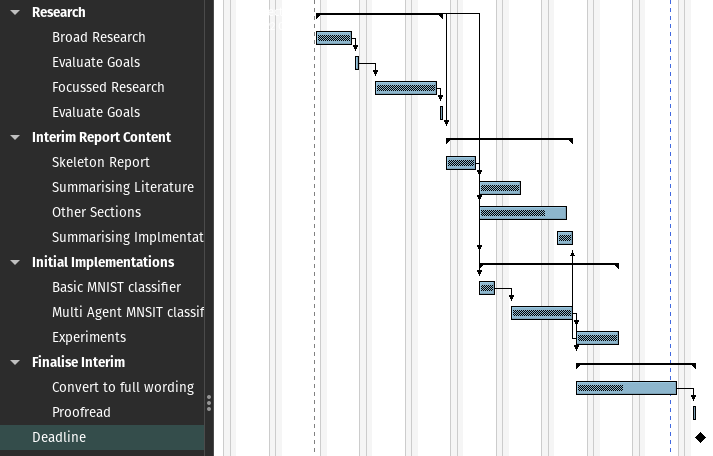
\includegraphics[width=\textwidth]{gantt_pre}



\section{Remaining Work}
A second Gantt chart was created for planning the project post-interim. This Gantt was made near the end of the first semester when a better understanding of the project had been developed through research. In this char, only two problems are planned for, as this has been decided to be the minimum problems require for the scope of the project. If these problems take less time than expected, further problems will be integrated into the development phase. There is also a large block of time allocated in the housekeeping phase to act as a buffer in case any other area of the project takes longer than expected. Ideally, the project will be handed in at the start of this period.

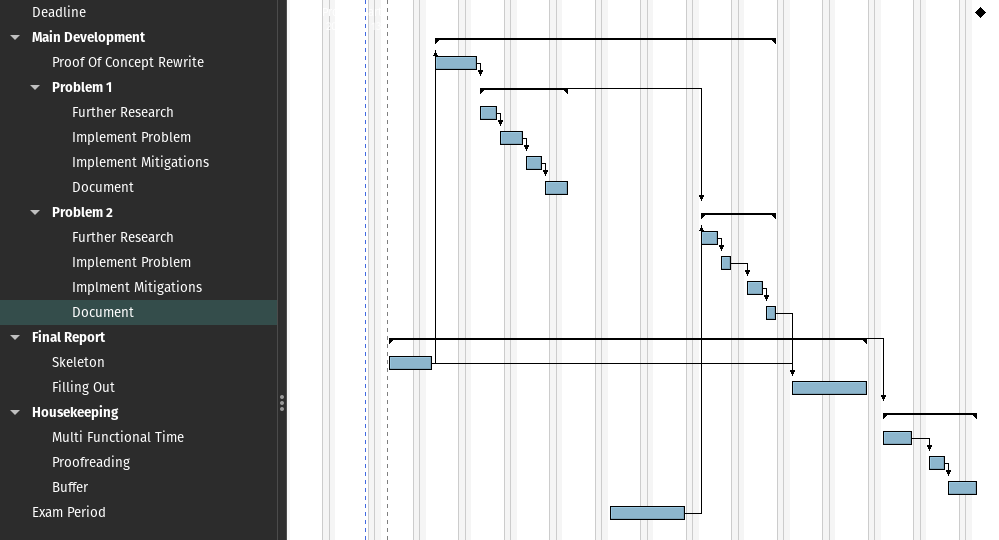
\includegraphics[width=\textwidth]{gantt_post}



\section{Risk Assessment}
\subsection{Personal Issues}

\subsubsection{Description}
This risk entails all personal issues which cause the author to be unable to do work, such as illness.

\subsubsection{Risk Calculations}
\emph{Severity (1-5):} 3 \\
\emph{Likelihood (1-5):} 3 \\
\emph{Overall Risk (1-25):} \textbf{9}

\subsubsection{Mitigation}
As many sections and modules as possible from the codebase will be designed to have minimal requirements from other sections. This means that, even if the author is unable to work for a period of time, some less important sections can be skipped with minimal effect on the reset of the project.

\subsection{Hardware Failure - Local Computer}
\subsubsection{Description}
This risk entails a failure on the authors local computer of any kind, such as a graphics card or storage breakage.

\subsubsection{Risk Calculations}
\emph{Severity (1-5):} 4 \\
\emph{Likelihood (1-5):} 2 \\
\emph{Overall Risk (1-25):} \textbf{8}

\subsubsection{Mitigation}
To mitigate storage based failures, the project will be regularly backed up to \emph{GitHub}. If a core component of the work computer breaks, the author has access to a personal laptop and the \emph{Zepler Labs}. The deep learning environment along with dependencies is backed up to the authors \emph{Google Drive} in the form of a docker image, so that switching to a new computer would be a smooth process.

\subsection{Hardware Failure - Iridis 5}
\subsubsection{Description}
This risk entails a failure on the \emph{Iridis 5 Compute Cluster} which prevents it from being accessed by the author.

\subsubsection{Risk Calculations}
\emph{Severity (1-5):} 4 \\
\emph{Likelihood (1-5):} 1 \\
\emph{Overall Risk (1-25):} \textbf{4}

\subsubsection{Mitigation}
\emph{Iridis 5} will play a key role in this project when simulating large numbers of agents at once. However, it is possible to simulate lower numbers (around 10) agents at the same time on the authors local machine with a basic dataset. This could be a temporary solution if \emph{Iridis 5} went down for a short time. However, for a more permanent solution, funding may be acquired from the university to run the project on a cluster of \emph{AWS} servers, as the author has some experience in that field. 

\subsection{Algorithm Fails to Work}
\subsubsection{Description}
This risk describes a situation where the algorithm of swarm learning does not function as well as expected. However, this is very unlikely as swarm learning has been proven to work in numerous papers CITE ME.

\subsubsection{Risk Calculations}
\emph{Severity (1-5):} 5 \\
\emph{Likelihood (1-5):} 1 \\
\emph{Overall Risk (1-25):} \textbf{5}

\subsubsection{Mitigation}
This is not an ideal situation, however it may be possible to shift the project away from swarm learning and onto federated learning. Federated learning is more commonly used and therefore has more literature, meaning that it is more likely to be an achievable goal to implement it. This would be a last resort though.